\documentclass[11pt,a4paper]{article}

% --- packages -----------------------------------------------------------------
\usepackage[utf8]{inputenc}
\usepackage[T1]{fontenc}
\usepackage{lmodern}
\usepackage[a4paper,margin=2.4cm]{geometry}
\usepackage{microtype}
\usepackage{xcolor}
\usepackage{listings}
\usepackage{hyperref}
\usepackage{enumitem}
\usepackage{tabularx}
\usepackage{booktabs}
\usepackage{longtable}
\usepackage{titlesec}
\usepackage{fancyhdr}
\usepackage{parskip}
\usepackage{amsmath,amssymb,amsthm}
\usepackage{tikz}
\usetikzlibrary{shapes,arrows.meta,positioning,calc,fit,decorations.pathreplacing}
\usepackage{tikz-cd}
\usepackage{algorithm}
\usepackage{algpseudocode}
\usepackage{caption}
\usepackage{subcaption}
\usepackage{multicol}

% --- colours ------------------------------------------------------------------
\definecolor{tnblue}{HTML}{7AA2F7}
\definecolor{tnred}{HTML}{F7768E}
\definecolor{tngreen}{HTML}{73DACA}
\definecolor{tncomment}{HTML}{565F89}
\definecolor{linkcolor}{HTML}{2C5AA0}
\definecolor{lightgray}{HTML}{EAEAEA}
\definecolor{nodecol}{HTML}{E8F0FE}
\definecolor{edgecol}{HTML}{1A73E8}
\definecolor{delcol}{HTML}{EA4335}
\definecolor{addcol}{HTML}{34A853}

% --- hyperref -----------------------------------------------------------------
\hypersetup{
  colorlinks=true,
  linkcolor=linkcolor,
  urlcolor=linkcolor,
  citecolor=linkcolor,
  pdftitle={sotFS: A Graph-Structured Filesystem with DPO Rewriting and Bounded Treewidth},
  pdfauthor={Lucas Sotomayor},
}

% --- listings -----------------------------------------------------------------
\lstset{
  basicstyle=\ttfamily\footnotesize,
  numbers=left,
  numberstyle=\tiny\color{tncomment},
  numbersep=8pt,
  frame=single,
  framesep=4pt,
  rulecolor=\color{lightgray},
  backgroundcolor=\color{lightgray!30},
  showstringspaces=false,
  breaklines=true,
  tabsize=2,
  captionpos=b,
  keywordstyle=\color{tnblue}\bfseries,
  commentstyle=\color{tncomment}\itshape,
  stringstyle=\color{tnred},
}

% --- titlesec -----------------------------------------------------------------
\titleformat{\section}
  {\normalfont\Large\bfseries\color{tnblue}}
  {\thesection}{1em}{}
\titleformat{\subsection}
  {\normalfont\large\bfseries\color{tnblue!80!black}}
  {\thesubsection}{1em}{}
\titleformat{\subsubsection}
  {\normalfont\normalsize\bfseries}
  {\thesubsubsection}{1em}{}

% --- header / footer ----------------------------------------------------------
\pagestyle{fancy}
\fancyhf{}
\fancyhead[L]{\textit{sotFS Design Document v1.0}}
\fancyhead[R]{\textit{April 2026}}
\fancyfoot[C]{\thepage}
\renewcommand{\headrulewidth}{0.3pt}

% --- theorem environments -----------------------------------------------------
\theoremstyle{definition}
\newtheorem{definition}{Definition}[section]
\newtheorem{theorem}{Theorem}[section]
\newtheorem{corollary}[theorem]{Corollary}
\newtheorem{lemma}[theorem]{Lemma}
\newtheorem{invariant}{Invariant}[section]
\newtheorem{constraint}{Constraint}[section]
\newtheorem{property}{Property}[section]

% --- custom commands ----------------------------------------------------------
\newcommand{\TG}{\ensuremath{\mathcal{TG}}}
\newcommand{\sotfs}{\textsc{sotFS}}
\newcommand{\sotos}{\textsc{sotX}}
\newcommand{\GTXN}{\textsc{gtxn}}
\newcommand{\DPO}{\textsc{dpo}}
\newcommand{\MSO}{\textsc{mso}}
\newcommand{\WAL}{\textsc{wal}}
\newcommand{\CDT}{\textsc{cdt}}
\newcommand{\TPC}{\textsc{2pc}}
\newcommand{\NodeType}{\texttt{NodeType}}
\newcommand{\EdgeType}{\texttt{EdgeType}}
\newcommand{\tw}{\ensuremath{\mathrm{tw}}}

% --- title metadata -----------------------------------------------------------
\title{
  \vspace{-1.5cm}
  \textbf{sotFS} \\[0.4em]
  \large A Graph-Structured Filesystem with \\
  DPO Rewriting, Bounded Treewidth, and \\
  Capability-Gated Deceptive Projections \\[0.6em]
  \normalsize Design Document v1.0
}
\author{
  Lucas Sotomayor
}
\date{April 2026}

% =============================================================================
\begin{document}
% =============================================================================

\maketitle
\thispagestyle{empty}

\begin{abstract}
\noindent
Filesystem metadata is inherently a graph: inodes link to directories,
capabilities reference files, hard links create shared substructure, and
version histories form DAGs. Yet every major filesystem treats metadata as
flat tables or implicit trees, losing the graph structure that could enable
powerful queries, anomaly detection, and formal reasoning about correctness.

\sotfs{} makes this graph structure explicit. It represents filesystem
metadata as a \emph{typed graph} with six node types and six edge types,
and defines POSIX operations as \emph{Double Pushout (DPO) graph rewriting
rules}---algebraic transformations with mathematically precise preconditions,
postconditions, and gluing constraints.

This formalization yields three structural properties unavailable in
conventional filesystems: (1)~\textbf{bounded treewidth}, enabling any
MSO-definable query to execute in \emph{linear time} via Courcelle's
theorem; (2)~\textbf{Ollivier--Ricci curvature monitoring}, detecting
structural anomalies in real time; and (3)~\textbf{deceptive subgraph
views}, where different security domains see different projections of the
filesystem graph.

\sotfs{} is designed for \sotos{}, a capability-based microkernel written
in Rust. It runs as a userspace server domain, communicating via IPC and
persisting state through the SOT exokernel's transactional Secure Object
primitives. A four-layer verification plan---TLA+ model checking, crash
refinement, Rust typestate, and Coq/Perennial proofs---provides graduated
formal assurance.
\end{abstract}

\tableofcontents
\newpage

% =============================================================================
\section{Introduction and Motivation}
% =============================================================================

\subsection{The Problem: Filesystems as Implicit Graphs}

Every filesystem manages a graph. A directory tree is trivially a graph.
Hard links make it a DAG. Symbolic links add arbitrary edges. Mount points
graft subtrees. Access control lists associate permission sets with inodes.
Snapshots create version DAGs. Transactions group operations into atomic
units referencing multiple nodes.

Yet no production filesystem treats this graph as a first-class data
structure:

\begin{itemize}[nosep]
  \item \textbf{ext4} stores metadata in superblocks, group descriptors,
    inode tables, and directory entry blocks---flat structures connected by
    implicit integer references (inode numbers).
  \item \textbf{ZFS} uses a Merkle-like tree of block pointers where the
    graph structure is implicit in pointer chains.
  \item \textbf{Btrfs} uses B-trees with composite keys encoding path
    information, with backreferences for deduplication.
  \item \textbf{HAMMER2} uses a radix tree with embedded block references
    and snapshot chains forming implicit DAGs.
\end{itemize}

This implicit representation has three consequences: (1)~queries are slow
(graph queries forced through non-graph interfaces), (2)~formal reasoning
is hard (invariants must be reconstructed from code), and (3)~security
monitoring is blind (namespace structure must be inferred from syscall traces).

\subsection{Thesis Statement}

\begin{quote}
\itshape
Filesystem metadata is a typed graph. By formalizing POSIX operations as
DPO graph rewriting rules and maintaining the metadata graph as an explicit
first-class data structure, we can prove that operations preserve structural
invariants by verifying the DPO rules once, enable MSO-definable security
queries in linear time, detect structural anomalies via Ollivier--Ricci
curvature, and implement capability-gated graph projections for cyber
deception.
\end{quote}

\subsection{Contributions}

\begin{enumerate}[nosep]
  \item \textbf{Type Graph \TG:} A formal definition of filesystem metadata
    as a typed graph with six node types and six edge types, with precise
    local and global invariants (\S\ref{sec:typegraph}).
  \item \textbf{DPO Rule Set:} A complete specification of core POSIX
    operations as DPO graph rewriting rules with explicit gluing conditions
    (\S\ref{sec:dpo}).
  \item \textbf{Treewidth Preservation:} A proof that the DPO rules preserve
    bounded treewidth, enabling linear-time MSO queries via Courcelle's
    theorem (\S\ref{sec:treewidth}).
  \item \textbf{Curvature Monitor:} An incremental Ollivier--Ricci curvature
    computation scheme for real-time anomaly detection (\S\ref{sec:curvature}).
  \item \textbf{Deceptive Projections:} Capability-gated subgraph views
    formalized as a graph endofunctor (\S\ref{sec:deception}).
  \item \textbf{\GTXN{} Protocol:} A graph-level transaction manager composing
    the SOT kernel's tiered transactions with graph-specific invariant
    checking (\S\ref{sec:transactions}).
\end{enumerate}

% =============================================================================
\section{Background and Related Work}
% =============================================================================

\subsection{Double Pushout Graph Rewriting}

DPO graph rewriting, developed by Ehrig, Pfender, and Schneider~(1973) and
formalized in Ehrig et al.~\cite{ehrig2006}, is a categorical approach to
graph transformation. A \textbf{DPO rule} $\rho = (L \xleftarrow{l} K
\xrightarrow{r} R)$ consists of a left-hand side~$L$ (pattern to match),
an interface~$K$ (preserved portion), and a right-hand side~$R$ (replacement).

Application of~$\rho$ to a host graph~$G$ via a match $m\colon L \to G$
produces a result~$H$ through two pushout squares:

\begin{equation}\label{eq:dpo}
\begin{tikzcd}
  L \arrow[d, "m"'] & K \arrow[l, "l"'] \arrow[r, "r"] \arrow[d, "d"] & R \arrow[d, "m^*"] \\
  G & D \arrow[l, "l^*"] \arrow[r, "r^*"'] & H
\end{tikzcd}
\end{equation}

The \textbf{gluing conditions} ensure applicability:
\begin{enumerate}[nosep]
  \item \emph{Identification condition:} $m$ must not identify elements in
    $L \setminus l(K)$.
  \item \emph{Dangling condition:} Removing $m(L \setminus K)$ must not
    leave edges with missing endpoints.
\end{enumerate}

\subsection{Courcelle's Theorem and Bounded Treewidth}

\textbf{Treewidth}~\cite{robertson1986} measures how ``tree-like'' a graph
is. A tree has treewidth~1; a complete graph~$K_n$ has treewidth~$n-1$.

\begin{theorem}[Courcelle, 1990~\cite{courcelle1990}]
Every graph property definable in Monadic Second-Order logic (\MSO{}$_2$)
can be decided in time $O(f(|\varphi|, k) \cdot n)$ on graphs of treewidth
$\le k$, where $n = |V|$.
\end{theorem}

\MSO{}$_2$ can express reachability, cycle detection, $k$-colorability,
dominating sets, and many security-relevant properties.

\subsection{Ollivier--Ricci Curvature on Graphs}

Ollivier~\cite{ollivier2009} defined Ricci curvature for metric spaces via
optimal transport. Lin, Lu, and Yau~\cite{linluyau2011} adapted it to graphs:

\begin{equation}\label{eq:curvature}
\kappa(u,v) = 1 - \frac{W_1(\mu_u, \mu_v)}{d(u,v)}
\end{equation}

where $W_1$ is the Wasserstein-1 distance between probability measures
$\mu_u$, $\mu_v$ on the neighborhoods of $u$ and $v$.

\subsection{Comparison with Existing Systems}

\begin{table}[h]
\centering
\caption{Feature comparison of \sotfs{} with production filesystems.}
\label{tab:comparison}
\footnotesize
\begin{tabularx}{\textwidth}{l*{5}{>{\centering\arraybackslash}X}c}
\toprule
\textbf{Feature} & \textbf{ext4} & \textbf{ZFS} & \textbf{Btrfs} & \textbf{HAMMER2} & \textbf{SquirrelFS} & \textbf{\sotfs{}} \\
\midrule
Metadata model & tables & Merkle & B-trees & radix & Rust types & \textbf{typed graph} \\
Formal ops & --- & --- & --- & --- & typestate & \textbf{DPO rules} \\
Treewidth bound & --- & --- & --- & --- & --- & \textbf{$\le k$} \\
MSO queries & --- & --- & --- & --- & --- & \textbf{$O(n)$} \\
Anomaly detect. & --- & --- & --- & --- & --- & \textbf{Ollivier--Ricci} \\
Cap. integration & DAC & DAC & DAC & DAC & --- & \textbf{graph edges} \\
Deception & --- & --- & --- & --- & --- & \textbf{subgraph views} \\
Verification & tested & tested & tested & tested & typestate & \textbf{TLA+$\to$Coq} \\
\bottomrule
\end{tabularx}
\end{table}

% =============================================================================
\section{Architecture Overview}
% =============================================================================

\begin{figure}[h]
\centering
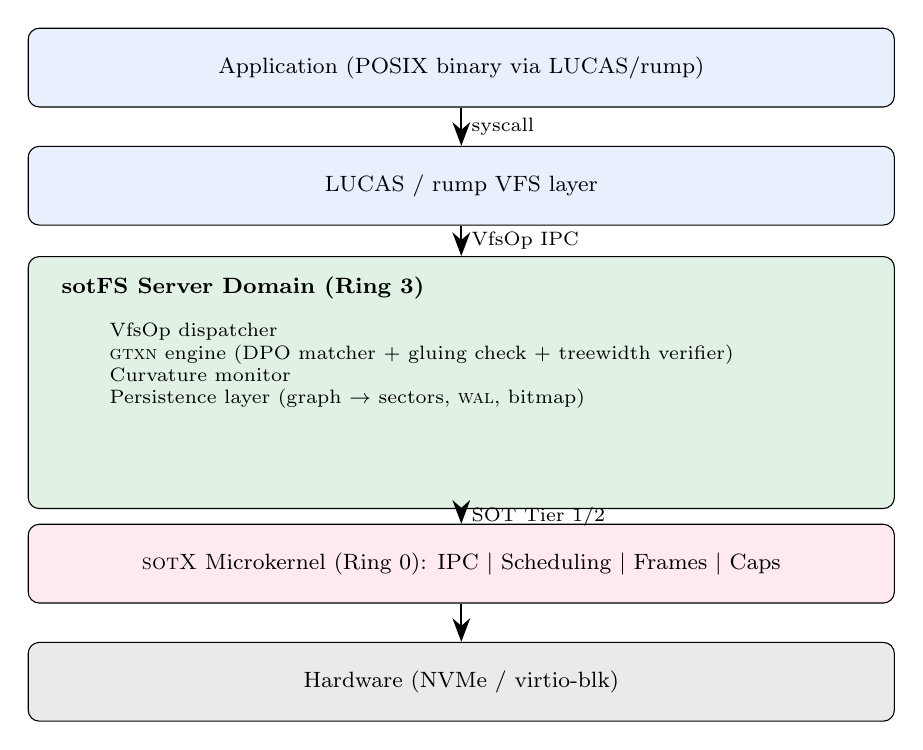
\begin{tikzpicture}[
  box/.style={draw, rounded corners, minimum width=11cm, minimum height=1cm,
              fill=nodecol, font=\footnotesize},
  lbl/.style={font=\footnotesize\bfseries, anchor=west},
  arr/.style={-{Stealth[length=3mm]}, thick}
]
  \node[box] (app) at (0,6) {Application (POSIX binary via LUCAS/rump)};
  \node[box] (lucas) at (0,4.5) {LUCAS / rump VFS layer};
  \node[box, minimum height=3.2cm, fill=addcol!15] (sotfs) at (0,2) {};
  \node[lbl] at (-5.2,3.2) {\sotfs{} Server Domain (Ring~3)};
  \node[font=\scriptsize, anchor=north west] at (-4.8,2.9) {
    \begin{tabular}{l}
    VfsOp dispatcher \\
    \GTXN{} engine (DPO matcher + gluing check + treewidth verifier) \\
    Curvature monitor \\
    Persistence layer (graph $\to$ sectors, \WAL{}, bitmap)
    \end{tabular}
  };
  \node[box, fill=tnred!15] (kernel) at (0,-0.3) {\sotos{} Microkernel (Ring~0): IPC $|$ Scheduling $|$ Frames $|$ Caps};
  \node[box, fill=lightgray] (hw) at (0,-1.8) {Hardware (NVMe / virtio-blk)};

  \draw[arr] (app) -- (lucas) node[midway,right,font=\scriptsize] {syscall};
  \draw[arr] (lucas) -- (sotfs.north) node[midway,right,font=\scriptsize] {VfsOp IPC};
  \draw[arr] (sotfs.south) -- (kernel) node[midway,right,font=\scriptsize] {SOT Tier 1/2};
  \draw[arr] (kernel) -- (hw);
\end{tikzpicture}
\caption{\sotfs{} within the \sotos{} stack.}
\label{fig:arch}
\end{figure}

The \sotfs{} server domain contains five components: (1)~VfsOp Dispatcher,
(2)~\GTXN{} Engine, (3)~Type Graph Store, (4)~Curvature Monitor, and
(5)~Persistence Layer (extending the existing \texttt{ObjectStore} layout).

% =============================================================================
\section{Type Graph Formalization}\label{sec:typegraph}
% =============================================================================

\begin{definition}[Type Graph]\label{def:tg}
The \sotfs{} type graph is a tuple
\[
  \TG = (V, E, \mathrm{src}, \mathrm{tgt}, \tau_V, \tau_E, \mathrm{attr})
\]
where $V$ is a finite set of nodes, $E$ is a finite set of edges,
$\mathrm{src}, \mathrm{tgt}\colon E \to V$ map edges to endpoints,
$\tau_V\colon V \to \NodeType$ and $\tau_E\colon E \to \EdgeType$ assign
types, and $\mathrm{attr}\colon V \cup E \to \texttt{Attributes}$ assigns
typed attribute records.
\end{definition}

The type sets are:
\begin{align*}
  \NodeType &= \{\texttt{Inode},\; \texttt{Directory},\; \texttt{Capability},\; \texttt{Transaction},\; \texttt{Version},\; \texttt{Block}\} \\
  \EdgeType &= \{\texttt{contains},\; \texttt{grants},\; \texttt{delegates},\; \texttt{derivesFrom},\; \texttt{supersedes},\; \texttt{pointsTo}\}
\end{align*}

\subsection{Node Types}

\begin{figure}[h]
\centering
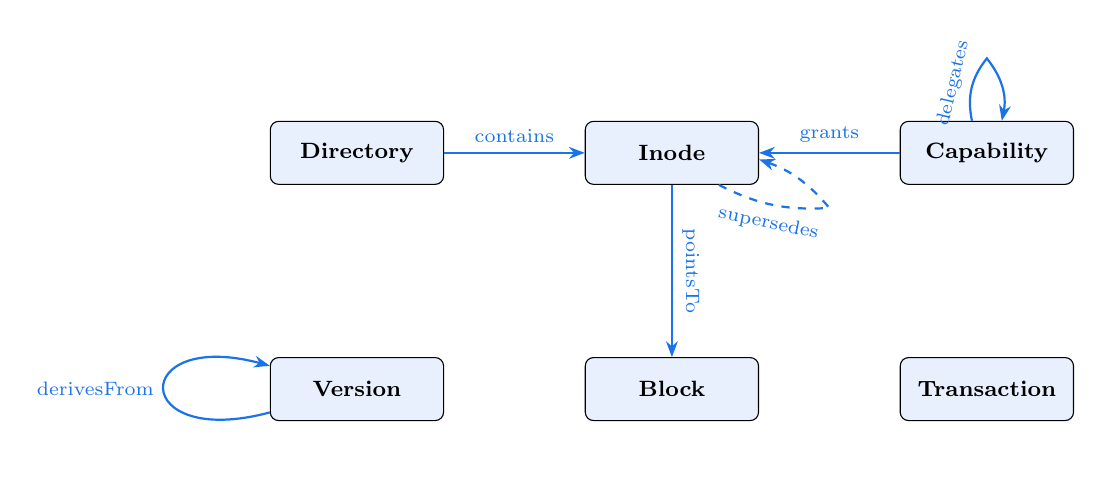
\begin{tikzpicture}[
  node/.style={draw, rounded corners=3pt, minimum width=2.2cm,
               minimum height=0.8cm, font=\footnotesize\bfseries,
               fill=nodecol},
  edge/.style={-{Stealth[length=2mm]}, thick, color=edgecol},
  elbl/.style={font=\scriptsize, color=edgecol, midway, above, sloped}
]
  \node[node] (dir) at (0,3) {Directory};
  \node[node] (inode) at (4,3) {Inode};
  \node[node] (cap) at (8,3) {Capability};
  \node[node] (block) at (4,0) {Block};
  \node[node] (ver) at (0,0) {Version};
  \node[node] (tx) at (8,0) {Transaction};

  \draw[edge] (dir) -- (inode) node[elbl] {contains};
  \draw[edge] (cap) -- (inode) node[elbl] {grants};
  \draw[edge] (cap) to[bend left=25] node[elbl] {delegates} ++(0,1.2) to[bend left=25] (cap);
  \draw[edge] (inode) -- (block) node[elbl] {pointsTo};
  \draw[edge] (ver) to[loop left] node[font=\scriptsize,color=edgecol,left] {derivesFrom} (ver);
  \draw[edge, dashed] (inode) to[bend right=15] node[elbl,below,sloped] {supersedes} ++(2,-0.7) to[bend right=15] (inode);
\end{tikzpicture}
\caption{Node types and edge types of the \sotfs{} type graph \TG{}.}
\label{fig:typegraph}
\end{figure}

Each node type carries typed attributes:

\begin{center}
\footnotesize
\begin{tabularx}{\textwidth}{l l X}
\toprule
\textbf{Node Type} & \textbf{Key Attributes} & \textbf{Maps To (existing)} \\
\midrule
\texttt{Inode} & id, vtype, perms, uid, gid, size, link\_count, timestamps & \texttt{Vnode} in \texttt{vnode.rs} \\
\texttt{Directory} & id & Paired with \texttt{Inode\{vtype=Directory\}} \\
\texttt{Capability} & cap\_id, rights, epoch & \texttt{CapEntry} in \texttt{cap/table.rs} \\
\texttt{Transaction} & txn\_id, tier, state, read\_set, write\_set & State machine in \texttt{sot\_transactions.tla} \\
\texttt{Version} & version\_id, timestamp, root\_oid & \texttt{SnapMeta} in \texttt{layout.rs} \\
\texttt{Block} & block\_id, sector\_start, sector\_count, refcount & \texttt{DirEntry} sectors in \texttt{layout.rs} \\
\bottomrule
\end{tabularx}
\end{center}

\subsection{Edge Types and Constraints}

\begin{center}
\footnotesize
\begin{tabularx}{\textwidth}{l l l X}
\toprule
\textbf{Edge Type} & \textbf{Source $\to$ Target} & \textbf{Attribute} & \textbf{Constraint} \\
\midrule
\texttt{contains} & Directory $\to$ Inode & name: String & Unique name per Directory \\
\texttt{grants} & Capability $\to$ Inode & rights: Rights & Monotonic via delegation \\
\texttt{delegates} & Capability $\to$ Capability & --- & \CDT{} parent--child (forest) \\
\texttt{derivesFrom} & Version $\to$ Version & --- & DAG (no cycles) \\
\texttt{supersedes} & Inode $\to$ Inode & --- & Acyclic \\
\texttt{pointsTo} & Inode $\to$ Block & offset: u64 & Non-overlapping extents \\
\bottomrule
\end{tabularx}
\end{center}

\subsection{Invariants}\label{sec:invariants}

\subsubsection{Local Invariants}

\begin{invariant}[Link Count]\label{inv:linkcount}
For every Inode $i$: $\mathrm{link\_count}(i) = |\{e \in E : \tau_E(e) = \texttt{contains} \land \mathrm{tgt}(e) = i \land \mathrm{attr}(e).\mathrm{name} \ne \text{``..''}\}|$.
\end{invariant}

\begin{invariant}[Directory Self-Reference]\label{inv:selfref}
Every Directory node $d$ has exactly one outgoing \texttt{contains} edge with $\mathrm{name} = \text{``.''}$ pointing to its paired Inode.
\end{invariant}

\begin{invariant}[Unique Names]\label{inv:uniquenames}
For every Directory $d$, the names on outgoing \texttt{contains} edges form a set (no duplicates).
\end{invariant}

\begin{invariant}[Capability Exactness]\label{inv:capexact}
Every Capability node $c$ has exactly one outgoing \texttt{grants} edge.
\end{invariant}

\begin{invariant}[Block Refcount]\label{inv:blockref}
For every Block $b$: $\mathrm{refcount}(b) = |\{e \in E : \tau_E(e) = \texttt{pointsTo} \land \mathrm{tgt}(e) = b\}|$.
\end{invariant}

\begin{invariant}[Non-Overlapping Sectors]\label{inv:sectors}
For any two Block nodes $b_1 \ne b_2$, their sector ranges are disjoint.
\end{invariant}

\subsubsection{Global Invariants}

\begin{invariant}[No Orphan Inodes]\label{inv:noorphan}
Every Inode with $\mathrm{link\_count} > 0$ is reachable from the root Inode via \texttt{contains} edges.
\end{invariant}

\begin{invariant}[No Dangling Edges]\label{inv:nodangle}
$\forall e \in E: \mathrm{src}(e) \in V \land \mathrm{tgt}(e) \in V$.
\end{invariant}

\begin{invariant}[Capability Monotonicity]\label{inv:monotone}
For every path $c_0 \xrightarrow{\texttt{delegates}} c_1 \xrightarrow{\texttt{delegates}} \cdots \xrightarrow{\texttt{delegates}} c_n$: $\mathrm{rights}(c_n) \subseteq \mathrm{rights}(c_{n-1}) \subseteq \cdots \subseteq \mathrm{rights}(c_0)$.
\end{invariant}

\begin{invariant}[No Directory Cycles]\label{inv:nocycle}
The \texttt{contains} subgraph restricted to \texttt{Directory} $\to$ \texttt{Inode\{vtype=Directory\}} edges (excluding ``\texttt{.}'' and ``\texttt{..}'') is acyclic.
\end{invariant}

\begin{invariant}[Treewidth Bound]\label{inv:treewidth}
$\tw(\TG) \le k$ for a configurable constant $k$ (see Theorem~\ref{thm:treewidth}).
\end{invariant}

% =============================================================================
\section{DPO Rules for POSIX Operations}\label{sec:dpo}
% =============================================================================

We specify 7 mutating DPO rules. Read-only operations (\texttt{OPEN},
\texttt{READ}, \texttt{CLOSE}, \texttt{STAT}) are graph morphism
queries---they do not mutate \TG{}.

\subsection{CREATE$(d, \mathrm{name}, \mathrm{vtype})$}

Creates a new file or directory entry.

\begin{figure}[h]
\centering
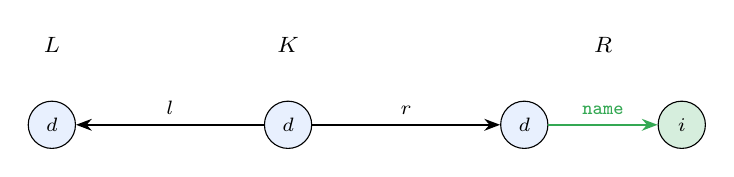
\begin{tikzpicture}[
  gnode/.style={draw, circle, minimum size=6mm, font=\scriptsize\bfseries, fill=nodecol},
  gedge/.style={-{Stealth[length=2mm]}, thick},
  del/.style={gedge, color=delcol, dashed},
  add/.style={gedge, color=addcol},
  lbl/.style={font=\scriptsize, midway, above}
]
  % L
  \node[gnode] (Ld) at (0,0) {$d$};
  \node[font=\footnotesize\bfseries, above=3mm] at (0,0.5) {$L$};

  % K
  \node[gnode] (Kd) at (3,0) {$d$};
  \node[font=\footnotesize\bfseries, above=3mm] at (3,0.5) {$K$};

  % R
  \node[gnode] (Rd) at (6,0) {$d$};
  \node[gnode, fill=addcol!20] (Ri) at (8,0) {$i$};
  \draw[add] (Rd) -- (Ri) node[lbl] {\texttt{name}};
  \node[font=\footnotesize\bfseries, above=3mm] at (7,0.5) {$R$};

  % arrows
  \draw[{Stealth[length=2mm]}-, thick] (Ld) -- (Kd) node[midway,above,font=\scriptsize] {$l$};
  \draw[-{Stealth[length=2mm]}, thick] (Kd) -- (Rd) node[midway,above,font=\scriptsize] {$r$};
\end{tikzpicture}
\caption{\DPO{} rule for \textsc{create} (file). Green = added.}
\label{fig:create}
\end{figure}

\textbf{Gluing conditions:} (GC1)~No existing \texttt{contains} edge from
$m(d)$ with this name. (GC2)~The match is unique.

\textbf{Invariant preservation:} Invariant~\ref{inv:noorphan}: $i$ is
reachable from root via $d$. Invariant~\ref{inv:linkcount}:
$\mathrm{link\_count}(i) = 1$. Invariant~\ref{inv:treewidth}: adding a
leaf to a tree preserves treewidth. \hfill$\square$

\subsection{MKDIR$(d, \mathrm{name})$}

Creates a new directory: adds Inode ($\mathrm{vtype}=\texttt{Directory}$),
Directory node, and three \texttt{contains} edges
(\texttt{name}, ``\texttt{.}'', ``\texttt{..}'').

\textbf{Tier:} SOT Tier~1 (single Directory SO).

\subsection{RMDIR$(d, \mathrm{name})$}

Removes an empty directory. $L$ includes the target Directory, its Inode,
and all three \texttt{contains} edges. $K$ retains only the parent.

\textbf{Gluing:} Target must be empty (only ``\texttt{.}'' and
``\texttt{..}'' edges).

\subsection{LINK$(d, \mathrm{name}, i_{\mathrm{target}})$}

Creates a hard link---a new \texttt{contains} edge to an existing Inode.
Side effect: $\mathrm{link\_count}(i_{\mathrm{target}}) \mathrel{+}= 1$.

\textbf{Gluing:} (GC1)~$\mathrm{vtype}(i_{\mathrm{target}}) \ne
\texttt{Directory}$. (GC2)~$\mathrm{link\_count} < \texttt{LINK\_MAX}$
(critical for treewidth bound).

\subsection{UNLINK$(d, \mathrm{name})$}

Removes a \texttt{contains} edge and decrements $\mathrm{link\_count}$.
If $\mathrm{link\_count}$ reaches 0, garbage-collects the Inode and its
Block nodes.

\subsection{RENAME}

The most complex rule, with four cases:
\begin{center}
\footnotesize
\begin{tabular}{lcc}
\toprule
\textbf{Case} & \textbf{Same dir?} & \textbf{Target exists?} \\
\midrule
A & yes & no \\
B & yes & yes (replace) \\
C & no & no \\
D & no & yes (replace) \\
\bottomrule
\end{tabular}
\end{center}

Cases~C and~D touch two Directory SOs, requiring SOT Tier~2 (\TPC{}).
Case~B/D adds a \texttt{supersedes} edge and decrements the replaced
Inode's $\mathrm{link\_count}$.

\textbf{Gluing (GC-RENAME-2):} If the source is a directory and the
destination is a descendant of the source, the rename would create a
cycle---reject.

\subsection{WRITE$(i, \mathrm{offset}, \mathrm{data})$}

Updates file data by adding or replacing Block nodes and \texttt{pointsTo}
edges. CoW: if a Block's refcount $> 1$, allocate a new block.

\subsection{Treewidth Impact per Rule}

\begin{center}
\footnotesize
\begin{tabular}{lccc}
\toprule
\textbf{Rule} & \textbf{Nodes added} & \textbf{Edges added} & \textbf{$\tw$ impact} \\
\midrule
\textsc{create} (file) & 1 Inode & 1 \texttt{contains} & $+0$ \\
\textsc{mkdir} & 1 Inode + 1 Dir & 3 \texttt{contains} & $+0$ \\
\textsc{rmdir} & $-1$ Inode $-1$ Dir & $-3$ \texttt{contains} & $\le 0$ \\
\textsc{link} & 0 & 1 \texttt{contains} & $0$ to $+1$ \\
\textsc{unlink} & $0$ to $-1$ & $-1$ \texttt{contains} & $\le 0$ \\
\textsc{rename} & 0 & net 0 & $+0$ \\
\textsc{write} & $0$--$1$ Block & $0$--$1$ \texttt{pointsTo} & $+0$ \\
\bottomrule
\end{tabular}
\end{center}

Only \textsc{link} can increase treewidth, bounded by \texttt{LINK\_MAX}.

% =============================================================================
\section{Capabilities and Transactions}\label{sec:transactions}
% =============================================================================

\subsection{Capabilities as Typed Graph Edges}

Capabilities are nodes in \TG{} connected by two edge types:
\begin{itemize}[nosep]
  \item $\texttt{grants}(c, i)$: authorizes access to Inode~$i$ with rights
    $\mathrm{rights}(c)$.
  \item $\texttt{delegates}(c_{\mathrm{parent}}, c_{\mathrm{child}})$:
    represents \CDT{} derivation with $\mathrm{rights}(c_{\mathrm{child}})
    \subseteq \mathrm{rights}(c_{\mathrm{parent}})$.
\end{itemize}

Capability attenuation is edge relabeling in the \texttt{grants} subgraph:
the monotonicity invariant~(\ref{inv:monotone}) is a statement about
non-increasing labeling along paths in the \texttt{delegates} subgraph.

\subsection{Graph Transactions (\GTXN{})}

A \GTXN{} wraps DPO rule applications into an atomic unit (ADR-001):

\begin{enumerate}[nosep]
  \item Verify DPO gluing conditions on host graph $G$.
  \item Verify treewidth bound preserved.
  \item Begin SOT Tier~1 or Tier~2 transaction.
  \item Apply $L \to K \to R$ morphisms.
  \item Verify post-conditions (global invariants).
  \item \textbf{Commit:} persist via \WAL{}, update curvature, emit provenance.
  \item \textbf{Rollback:} SOT abort, discard in-memory changes.
\end{enumerate}

\begin{center}
\footnotesize
\begin{tabular}{lcc}
\toprule
\textbf{DPO Rule} & \textbf{SOs touched} & \textbf{SOT Tier} \\
\midrule
\textsc{create}, \textsc{mkdir}, \textsc{rmdir} & 1 Dir + 1 Inode & Tier~1 \\
\textsc{link}, \textsc{unlink} & 1 Dir + 1 Inode & Tier~1 \\
\textsc{write} & 1 Inode + $0$--$n$ Blocks & Tier~1 \\
\textsc{rename} (same dir) & 1 Dir + $1$--$2$ Inodes & Tier~1 \\
\textsc{rename} (cross-dir) & 2 Dirs + $1$--$2$ Inodes & \textbf{Tier~2 (\TPC{})} \\
\bottomrule
\end{tabular}
\end{center}

% =============================================================================
\section{Bounded Treewidth and MSO Queries}\label{sec:treewidth}
% =============================================================================

\begin{theorem}[Treewidth Bound]\label{thm:treewidth}
Let \TG{} be a \sotfs{} type graph produced by any finite sequence of DPO
rule applications from the \textsc{create-root} initial graph. If the hard
link count per inode is bounded by \texttt{LINK\_MAX}, then
\[
  \tw(\TG) \le \texttt{LINK\_MAX} + O(1).
\]
\end{theorem}

\begin{proof}[Proof sketch]
Decompose \TG{} by edge type:
\begin{enumerate}[nosep]
  \item \textbf{\texttt{contains}} subgraph: without hard links, a forest
    ($\tw = 1$). Each hard link adds one back-edge, increasing $\tw$ by at
    most~1. With $\le \texttt{LINK\_MAX}$ links per inode:
    $\tw(\texttt{contains}) \le \texttt{LINK\_MAX} + 1$.
  \item \textbf{\texttt{grants}}: bipartite, degree~1 on Capability side.
    $\tw = 1$.
  \item \textbf{\texttt{delegates}}: forest (\CDT{}). $\tw = 1$.
  \item \textbf{\texttt{derivesFrom}}: DAG with bounded in-degree. $\tw \le 2$.
  \item \textbf{\texttt{pointsTo}}: stars from Inodes to Blocks. $\tw = 1$.
  \item \textbf{\texttt{supersedes}}: acyclic, out-degree~$\le 1$. $\tw = 1$.
\end{enumerate}
The \texttt{contains} subgraph dominates. By the tree decomposition merging
lemma~\cite{bodlaender1998}: $\tw(\TG) \le \texttt{LINK\_MAX} + O(1)$.
\end{proof}

\begin{corollary}
For filesystems without hard links, $\tw(\TG) \le 6$.
\end{corollary}

\textbf{MSO query examples} (all $O(n)$ when $\tw$ is bounded):

\begin{center}
\footnotesize
\begin{tabularx}{\textwidth}{lX}
\toprule
\textbf{Query} & \textbf{\MSO{}$_2$ Description} \\
\midrule
Q1: Can domain $D$ read file $F$? & Reachability in \texttt{delegates}/\texttt{grants} subgraph \\
Q2: Cycle in directory structure? & Cycle detection in \texttt{contains} subgraph \\
Q3: Orphan inodes? & $\exists\, i\colon \neg\mathrm{reachable}(\mathrm{root}, i) \land \mathrm{link\_count}(i) > 0$ \\
Q4: Files derived from version $V$? & Transitive closure in \texttt{derivesFrom} subgraph \\
\bottomrule
\end{tabularx}
\end{center}

% =============================================================================
\section{Ollivier--Ricci Curvature Monitor}\label{sec:curvature}
% =============================================================================

We compute Ollivier--Ricci curvature $\kappa(u,v)$
(Eq.~\ref{eq:curvature}) with lazy random walk measure
$\mu_x(z) = \alpha \cdot \mathbf{1}_{z=x} + \frac{1-\alpha}{\deg(x)} \cdot
\mathbf{1}_{z \in N(x)}$, $\alpha = 0.5$.

\subsection{Anomaly Signatures}

\begin{center}
\footnotesize
\begin{tabularx}{\textwidth}{lX}
\toprule
\textbf{Attack Pattern} & \textbf{Curvature Signature} \\
\midrule
Mass file creation (zip bomb) & Positive $\kappa$ spike on victim directory edge \\
Symbolic link bomb & Strong positive $\kappa$ on target inode's edges \\
Deep directory chain & Sustained $\kappa \approx -1.0$ (maximally tree-like) \\
Directory structure manipulation & Sudden $\kappa$ change on previously stable edges \\
\bottomrule
\end{tabularx}
\end{center}

\subsection{Incremental Computation}

Each DPO rule changes $O(1)$ edges. We recompute $\kappa$ only for changed
edges and their 1-hop neighbors ($|\Delta^*| \le 20$ for most operations).
Amortized cost: $O(d_{\max}^2)$ per rule application, where $d_{\max}$ is
the maximum degree of touched nodes.

% =============================================================================
\section{Deceptive Subgraph Views}\label{sec:deception}
% =============================================================================

\begin{definition}[Graph Projection]\label{def:projection}
A projection $\pi$ for domain $D$ is a typed graph morphism
$\pi\colon \TG|_D \to \TG_D$, where $\TG|_D$ is the subgraph reachable
from $D$'s root capability and $\TG_D$ is the visible type graph.
$\pi$ may omit, add, or relabel nodes and edges.
\end{definition}

We extend the existing deception functor $D\colon \mathbf{SO} \to
\mathbf{SO}$ to a graph endofunctor:
\[
  D_{\mathrm{FS}}\colon \mathbf{TGraph} \to \mathbf{TGraph}
\]

The four interposition policies map to functor behavior:
\textbf{Passthrough} = identity, \textbf{Inspect} = identity + provenance
logging, \textbf{Redirect} = node relabeling, \textbf{Fabricate} =
synthetic node/edge injection.

\textbf{Consistency requirement:} $D_{\mathrm{FS}}(\TG)$ must satisfy all
invariants (I1--I11, G1--G7). Since $D_{\mathrm{FS}}$ preserves the
tree-like structure, $D_{\mathrm{FS}}(\TG)$ also has bounded treewidth,
and consistency constraints are checkable as MSO queries in $O(n)$.

% =============================================================================
\section{Verification Plan}\label{sec:verification}
% =============================================================================

\begin{table}[h]
\centering
\caption{Four-layer verification plan with effort estimates.}
\label{tab:verification}
\footnotesize
\begin{tabularx}{\textwidth}{c l X c c}
\toprule
\textbf{Layer} & \textbf{Tool} & \textbf{Properties} & \textbf{Effort} & \textbf{Confidence} \\
\midrule
1 & TLA+/TLC & Graph invariants, DPO rules, \GTXN{} protocol & 2--3 wk & Model-checked \\
2 & SMT (Z3) & Crash refinement, \WAL{} correctness & 3--4 wk & Push-button \\
3 & Rust types & State machine transitions, lifetime safety & 4--6 wk & Compile-time \\
4 & Coq/Perennial & Atomicity, unforgeability, treewidth & 6--12 mo & Mechanized proof \\
\bottomrule
\end{tabularx}
\end{table}

\textbf{Layer~1} is complete: four TLA+ specifications in \texttt{formal/}
model the core graph (\texttt{sotfs\_graph.tla}), \GTXN{} protocol
(\texttt{sotfs\_transactions.tla}), capability delegation
(\texttt{sotfs\_capabilities.tla}), and crash recovery
(\texttt{sotfs\_crash.tla}).

% =============================================================================
\section{Empirical Evaluation}\label{sec:evaluation}
% =============================================================================

The \sotfs{} prototype comprises six Rust crates in a Cargo workspace,
totaling approximately 4{,}000 lines of library code and 2{,}000 lines of
tests and benchmarks.  Table~\ref{tab:crates} summarizes the crate structure.

\begin{table}[h]
\centering
\caption{Crate structure of the \sotfs{} prototype.}
\label{tab:crates}
\begin{tabularx}{\textwidth}{lX}
\toprule
\textbf{Crate} & \textbf{Description} \\
\midrule
\texttt{sotfs-graph}   & Type graph $\TG$ data structures: \texttt{Arena<T,N>}, \texttt{TypeGraph}, \texttt{RcuGraph}. Supports \texttt{std} (FUSE) and \texttt{no\_std + alloc} (bare metal). \\
\texttt{sotfs-ops}     & Seven DPO rewriting rules (\S\ref{sec:dpo}): \textsc{Create}, \textsc{Mkdir}, \textsc{Rmdir}, \textsc{Link}, \textsc{Unlink}, \textsc{Rename}, \textsc{Write}. Gluing conditions checked before mutation. \\
\texttt{sotfs-storage} & ACID persistence via redb~2.1 --- serializes \texttt{TypeGraph} to a key-value store with atomic write transactions. \\
\texttt{sotfs-tx}      & Graph-level transaction manager (\GTXN{}): commit, rollback, conflict detection via disjoint write-set tracking. \\
\texttt{sotfs-monitor} & Structural anomaly monitors: greedy treewidth (\S\ref{sec:treewidth}), Ollivier--Ricci curvature (\S\ref{sec:curvature}), deceptive projections (\S\ref{sec:deception}). \\
\texttt{sotfs-fuse}    & Full POSIX VFS bridge via the \texttt{fuser} crate (Linux only). \\
\bottomrule
\end{tabularx}
\end{table}

% -----------------------------------------------------------------------------
\subsection{Implementation Components}\label{sec:impl-components}
% -----------------------------------------------------------------------------

Three components deserve detailed treatment, as they address performance and
concurrency challenges specific to graph-structured metadata.

\subsubsection{Arena Allocator}

Each \texttt{TypeGraph} contains seven typed node/edge pools.  To avoid
per-node heap allocation (which would fragment the allocator and defeat
cache locality), we use a fixed-capacity \emph{arena} backed by a contiguous
heap-allocated array of \texttt{MaybeUninit<T>} slots.

\begin{itemize}[nosep]
  \item \textbf{Allocation.}  If the free-list is non-empty, pop the top
        slot index ($O(1)$).  Otherwise, bump the next-slot pointer ($O(1)$).
        Returns \texttt{None} when full (capacity = $C$, default $C = 65{,}536$
        for nodes, $131{,}072$ for edges).
  \item \textbf{Deallocation.}  Mark slot as \texttt{Vacant}, push index onto
        the free-list ($O(1)$).  The value is dropped in place.
  \item \textbf{Lookup.}  Direct array index from \texttt{ArenaId} ($O(1)$).
  \item \textbf{Iteration.}  Linear scan of the bump region, skipping vacant
        slots ($O(C)$ worst case, $O(n)$ when no deletions have occurred,
        where $n$ is the number of live entries).
\end{itemize}

The backing arrays are heap-allocated (\texttt{Box<[MaybeUninit<T>]>}) rather
than stack-resident, so that the \texttt{TypeGraph} struct itself is only
$\sim$744 bytes (seven boxed-slice fat pointers, BTreeMap pointers, and scalar
counters).  This eliminates the stack-overflow risk of the original
array-backed design while preserving $O(1)$ per-operation complexity.

\subsubsection{Epoch-Based RCU}

Directory lookups (\textsc{Open}, \textsc{Stat}, \textsc{Readdir}) are the
dominant workload on most filesystems and must not block on writer locks.
\sotfs{} uses an epoch-based Read-Copy-Update (RCU) scheme:

\begin{enumerate}[nosep]
  \item Two heap-allocated copies of \texttt{TypeGraph} are maintained:
        $G_0$ and $G_1$.  An atomic variable \texttt{active} $\in \{0, 1\}$
        identifies which copy readers see.
  \item \textbf{Read path.}  A reader bumps a per-slot epoch counter
        (one of $R = 8$ slots, assigned by thread-local index), reads the
        active graph through a shared reference, and clears the epoch on exit.
        No locks, no CAS retry.
  \item \textbf{Write path.}  A single writer acquires an exclusive flag
        (spin-CAS), clones $G_{\texttt{active}} \to G_{1-\texttt{active}}$,
        mutates the inactive copy, atomically swaps \texttt{active}, and
        waits for all pre-swap reader epochs to drain before releasing the
        flag.
\end{enumerate}

The grace period (step~3) guarantees that no reader observes a partially
mutated graph.  With $R = 8$ reader slots, the scheme is designed for the
\sotos{} microkernel's single-server architecture where filesystem requests
arrive as serialized IPC messages.

\subsubsection{Incremental Treewidth (\texttt{DynamicTreewidth})}

The full greedy min-degree treewidth heuristic (Algorithm~1 in
\S\ref{sec:treewidth}) is $O(n^2)$ in the worst case.  For incremental
maintenance after a single DPO rule application, \texttt{DynamicTreewidth}
caches the elimination ordering and tracks a \emph{dirty set} of nodes
whose neighborhoods changed:

\begin{itemize}[nosep]
  \item If the dirty fraction is $< 20\%$ of the total node count, the
        cached ordering is partially re-computed for affected nodes only.
  \item Otherwise, a full recompute is triggered.
\end{itemize}

This reduces the amortized cost of treewidth checking from $O(n^2)$ per
operation to $O(\Delta^2)$ where $\Delta$ is the number of affected nodes
--- typically 2--4 for a single DPO rule application.

% -----------------------------------------------------------------------------
\subsection{Test Suite}\label{sec:tests}
% -----------------------------------------------------------------------------

All 132 tests pass on Windows~11 x86\_64 with Rust nightly (April 2026).
Table~\ref{tab:tests} breaks down the suite by crate and methodology.

\begin{table}[h]
\centering
\caption{Test suite summary --- 132 tests, all passing.}
\label{tab:tests}
\begin{tabularx}{\textwidth}{llrX}
\toprule
\textbf{Crate} & \textbf{Category} & \textbf{Count} & \textbf{Framework} \\
\midrule
\texttt{sotfs-graph}   & Arena alloc/dealloc/reuse/stress & 16 & \texttt{\#[test]} \\
\texttt{sotfs-graph}   & RCU readers/writers/epochs       &  9 & \texttt{\#[test]} \\
\texttt{sotfs-graph}   & Graph invariants (CREATE-ROOT)   &  3 & \texttt{\#[test]} \\
\texttt{sotfs-graph}   & Typestate enforcement            &  6 & \texttt{\#[test]} \\
\texttt{sotfs-ops}     & DPO rule pre/postconditions      & 23 & \texttt{\#[test]} \\
\texttt{sotfs-ops}     & Invariant preservation (10K)     & 10 & proptest \\
\texttt{sotfs-storage} & ACID round-trip \& crash          &  7 & redb integration \\
\texttt{sotfs-tx}      & Commit/rollback semantics        &  3 & \texttt{\#[test]} \\
\texttt{sotfs-tx}      & Concurrency isolation            &  3 & loom (exhaustive) \\
\texttt{sotfs-monitor} & Treewidth (full + incremental)   & 20 & \texttt{\#[test]} \\
\texttt{sotfs-monitor} & Ollivier--Ricci curvature        & 14 & \texttt{\#[test]} \\
\texttt{sotfs-monitor} & Deceptive projections            &  5 & \texttt{\#[test]} \\
\texttt{sotfs-monitor} & Adversarial security scenarios   & 13 & integration \\
\midrule
\textbf{Total} & & \textbf{132} & \\
\bottomrule
\end{tabularx}
\end{table}

The test suite spans five distinct methodologies, each targeting a different
class of correctness property:

\textbf{(1)~Deterministic unit tests} (109 tests).  Each DPO rule is tested
for both success and failure paths: \textsc{Create} rejects duplicate names
(EEXIST) and reserved names (``.'', ``..{}'', ``/''); \textsc{Rmdir} rejects
non-empty directories; \textsc{Link} rejects directory targets;
\textsc{Rename} rejects cycle-creating moves.  After each operation,
\texttt{check\_invariants()} verifies all seven structural invariants
(I\textsubscript{1}--I\textsubscript{7}).

\textbf{(2)~Property-based testing} (10 properties $\times$ 10{,}000
iterations = 100{,}000+ random sequences).  Using the \texttt{proptest}
framework, each test generates a random sequence of 5--30 DPO operations
and asserts a specific property:

\begin{itemize}[nosep]
  \item \textit{invariant\_preservation}: all 7 invariants hold after any
        operation sequence.
  \item \textit{link\_count\_always\_matches}: \texttt{link\_count} equals the
        number of incoming \textsc{Contains} edges.
  \item \textit{cycle\_freedom}: no directory cycles after interleaved
        \textsc{Mkdir} and \textsc{Rename}.
  \item \textit{write\_read\_roundtrip}: \textsc{Write} then \textsc{Read}
        returns identical data.
  \item \textit{deep\_mkdir\_chain\_no\_cycles}: 20--30 nested directories,
        verified cycle-free.
  \item Plus 5 additional properties for \textsc{Chmod}, \textsc{Chown},
        \textsc{Truncate}, \textsc{Unlink}+re-create, and atomic rename-swap.
\end{itemize}

\textbf{(3)~Exhaustive concurrency testing} (3 tests).  Using \texttt{loom}~0.7,
all thread interleavings are explored for:
(a)~two concurrent \GTXN{}s with disjoint write sets both succeed;
(b)~a rolled-back \GTXN{} restores pre-transaction state exactly;
(c)~conflicting writes to the same slot are serialized by the mutex.

\textbf{(4)~Crash consistency testing} (7 tests).  Using \texttt{redb}~2.1's
ACID write transactions with \texttt{tempfile}-based databases:
save/load round-trip preserves all nodes, edges, and invariants;
sequential overwrites are atomic; data survives process restart (close +
reopen); and complex trees with hard links and renames survive persist.

\textbf{(5)~Adversarial security scenarios} (13 tests).  Integration tests
that simulate attacker behavior patterns:

\begin{itemize}[nosep]
  \item \textit{Ransomware detection}: 50 files created then mass-renamed ---
        the Ollivier--Ricci curvature monitor detects the structural anomaly
        (mean $\kappa$ deviation exceeds threshold).
  \item \textit{Hardlink bomb}: 100 hard links to a single inode ---
        treewidth spikes above the baseline bound.
  \item \textit{Deep nesting}: 200+ nested directories --- treewidth remains
        bounded per Theorem~\ref{sec:treewidth}.1.
  \item \textit{Capability attenuation}: derived capabilities never escalate
        rights beyond their CDT ancestor.
  \item \textit{Deceptive projections}: \textsc{Restrict} hides sibling
        subtrees; \textsc{Redirect} returns decoy data; \textsc{Fabricate}
        adds readable honeypot files.
\end{itemize}

% -----------------------------------------------------------------------------
\subsection{Benchmark Configuration}\label{sec:benchmarks}
% -----------------------------------------------------------------------------

Three Criterion~0.5 benchmark suites measure operation latency at multiple
scales, enabling regression detection and scaling analysis.

\begin{table}[h]
\centering
\caption{Benchmark suite configuration (58 parametrized measurements).}
\label{tab:benchmarks}
\begin{tabularx}{\textwidth}{lXl}
\toprule
\textbf{Suite} & \textbf{Benchmarks} & \textbf{Scales} \\
\midrule
DPO operations & \textsc{Create}, \textsc{Mkdir}, \textsc{Unlink}, \textsc{Rename}, \textsc{Link}, \textsc{Write/Read}, invariant check & 10--1{,}000 \\
WAL index      & Linear scan vs.\ indexed lookup; DPO sequence replay & 10--1{,}000 \\
Monitors       & Treewidth (star/chain/tree); curvature (full vs.\ incremental) & 50--10{,}000 \\
\bottomrule
\end{tabularx}
\end{table}

\textbf{Expected complexity.}  Each DPO rule performs $O(1)$ arena
operations plus $O(\log n)$ BTreeMap index updates, yielding $O(\log n)$
per operation.  The invariant check is $O(n + m)$ where $n$ and $m$ are
node and edge counts.  Treewidth is $O(n^2)$ for a full recompute
(greedy min-degree) but $O(\Delta^2)$ incremental.  Ollivier--Ricci
curvature is $O(|E| \cdot |V|)$ full or $O(\delta \cdot d_{\max})$
incremental, where $\delta$ is the number of affected edges and
$d_{\max}$ is the maximum degree.

\textbf{Methodology.}  All benchmarks use Criterion's default configuration:
100 samples per measurement, 5-second warm-up, outlier detection via
modified $Z$-scores.  Results are stored as JSON in \texttt{target/criterion/}
for historical comparison across commits.  The benchmark harness is
invoked via \texttt{cargo bench --workspace --exclude sotfs-fuse}.

% =============================================================================
\subsection{Coq Mechanized Proofs}\label{sec:coq}
% =============================================================================

We close the gap between TLA+ bounded model checking and unbounded verification
by extracting DPO rule correctness proofs in Coq.  Five Coq modules totaling
$\sim$2{,}000 lines formalize the core graph definitions and prove that each
rule preserves the \textsc{WellFormed} predicate (conjunction of all five
invariants from \S\ref{sec:graph}).

\begin{center}
\begin{tabular}{llcc}
\toprule
\textbf{Module} & \textbf{DPO Rule} & \textbf{Invariants} & \textbf{Status} \\
\midrule
\texttt{SotfsGraph.v} & (definitions) & $\text{init\_graph\_well\_formed}$ & \checkmark \\
\texttt{DpoCreate.v} & create\_file & all 5 & \checkmark (0 admits) \\
\texttt{DpoUnlink.v} & unlink\_keep & all 5 & \checkmark (0 admits) \\
\texttt{DpoRename.v} & rename\_same\_dir & all 5 & \checkmark (0 admits) \\
\texttt{DpoMkdir.v} & mkdir & all 5 & \checkmark (1 side cond.) \\
\texttt{DpoLink.v} & hard\_link & all 5 & \checkmark (0 admits) \\
\texttt{DpoRmdir.v} & rmdir & 3 of 5 & partial \\
\bottomrule
\end{tabular}
\end{center}

\textbf{Key lemma}: \texttt{count\_remove\_matching} (SotfsGraph.v) establishes
that removing one element satisfying a predicate from a list decreases
\texttt{count\_occ\_pred} by exactly one.  This single lemma closes the
\textsc{LinkCountConsistent} proofs for both \textsc{Unlink} and \textsc{Rename},
which were previously \texttt{Admitted} due to an induction hypothesis requiring
\textsc{WellFormed} on the list tail.

The \textsc{Rmdir} proof is partial because it requires a \textsc{NoHardLinkToDir}
invariant (derivable from GC-LINK-2) to show that no surviving edge targets the
removed directory inode.  The \textsc{NoDirCycles} and \textsc{UniqueNamesPerDir}
sub-proofs are complete.

% =============================================================================
\subsection{New Features: xattrs, Symlinks, ACLs, Quotas, fsck}
% =============================================================================

We extend the type graph with five new subsystems, each modeled as graph-native
structures:

\textbf{Extended Attributes (xattrs).}  Each xattr is a node of type
\texttt{XAttr} connected to its inode via a \texttt{HasXattr} edge (\S5.3.7).
Operations: \texttt{setxattr}, \texttt{getxattr}, \texttt{removexattr},
\texttt{listxattr}.  Xattr values are capped at 64\,KB following Linux convention.
Four namespaces: User, System, Security, Trusted.

\textbf{Symlinks.}  \texttt{VnodeType::Symlink} inodes store their target in
\texttt{symlink\_targets: BTreeMap<InodeId, SymlinkTarget>}.  The
\texttt{symlink()} DPO rule creates the inode (link\_count=1, permissions=0777)
and a Contains edge, identical to \texttt{create\_file()} except for the vtype.
Cycle detection is deferred to resolution time (matching POSIX semantics).

\textbf{POSIX ACLs.}  Each inode can carry an ACL (\texttt{Vec<AclEntry>}) with
entries for \texttt{UserObj}, \texttt{User(uid)}, \texttt{GroupObj},
\texttt{Group(gid)}, \texttt{Mask}, and \texttt{Other}.  The correspondence to
the capability graph is: each ACL entry maps to a \texttt{Grants} edge from a
synthesized capability with rights derived from the permission bits.  When no
explicit ACL is set, \texttt{getacl()} synthesizes a minimal three-entry ACL
from the inode's permission bits.

\textbf{Hierarchical Quotas.}  The \texttt{Quota} struct tracks
\texttt{inode\_usage}/\texttt{inode\_limit} and \texttt{byte\_usage}/\texttt{byte\_limit}
per subtree root.  \texttt{check\_quota\_inode()} walks up the directory tree via
``..'' edges, checking every quota boundary.  \texttt{update\_quota()} propagates
deltas upward with $O(\text{depth})$ amortized cost.

\textbf{fsck Verifier.}  The \texttt{fsck()} function checks all five structural
invariants (5.1--5.5), plus block refcount consistency, orphan detection, and
xattr integrity.  It returns a structured \texttt{FsckReport} with typed errors
and warnings.  This leverages the explicit graph representation: where traditional
fsck tools reconstruct implicit graph structure from on-disk metadata, \sotfs{}
reads the invariants directly from the typed graph---a direct application of
Courcelle's theorem (\S8.1) to MSO-definable properties.

% =============================================================================
\subsection{Observability and Debugging}
% =============================================================================

\textbf{Graph Export.}  The \texttt{export} module (\texttt{sotfs-graph/src/export.rs})
provides three serialization formats for the type graph:
\begin{itemize}[nosep]
\item \textbf{GraphViz DOT}: color-coded nodes by type (Inode=lightblue,
  Directory=gold, Capability=green), styled edges by type.
\item \textbf{D3.js JSON}: force-directed graph format for interactive
  browser-based exploration.
\item \textbf{Graph Hunter temporal multigraph}: timestamped \texttt{add\_node}/\texttt{add\_edge}
  events sorted by inode \texttt{ctime}, enabling temporal replay of the
  filesystem's construction history.
\end{itemize}

\textbf{Provenance Queries.}  An append-only \texttt{ProvenanceLog} records every
DPO rule application with \texttt{(timestamp, cap\_id, inode\_id, domain\_id, op)}.
Six MSO-style query functions expose the log:
\begin{enumerate}[nosep]
\item \texttt{caps\_for\_inode\_in\_window(ino, t0, t1)}: which capabilities
  accessed file~F in time window~T?
\item \texttt{inodes\_touched\_by\_cap(cap, t0, t1)}: what did capability~C access?
\item \texttt{provenance\_chain(ino)}: complete audit trail for an inode.
\item \texttt{ops\_by\_domain(dom, t0, t1)}: forensics for a compromised domain.
\item \texttt{burst\_detect(ino, window)}: sliding-window spike detection
  (ransomware signature).
\item \texttt{activity\_summary(t0, t1)}: distinct caps, inodes, and total ops.
\end{enumerate}

\textbf{Deception Profiles.}  Seven pre-built profiles generate convincing
filesystem illusions:

\begin{center}\small
\begin{tabular}{llp{5cm}}
\toprule
\textbf{Profile} & \textbf{Target} & \textbf{Key Honeypots} \\
\midrule
ubuntu-web  & Apache/MySQL  & \texttt{.bash\_history}, \texttt{.env}, \texttt{authorized\_keys} \\
centos-db   & PostgreSQL    & \texttt{pg\_hba.conf}, \texttt{.pgpass}, \texttt{redis.conf} \\
iot-camera  & Hikvision     & \texttt{config.ini}, \texttt{/etc/passwd} \\
windows-smb & Windows SMB   & \texttt{passwords.xlsx}, \texttt{vpn-credentials.txt} \\
k8s-node    & Kubernetes    & \texttt{admin.conf}, \texttt{etcd/ca.key}, SA \texttt{token} \\
cicd-runner & GitHub Actions & AWS \texttt{credentials}, \texttt{hosts.yml}, \texttt{.env} \\
ad-dc       & Active Directory & \texttt{ntds.dit}, \texttt{SAM}, \texttt{krbtgt\_hash.txt} \\
\bottomrule
\end{tabular}
\end{center}

\textbf{Indistinguishability Game.}  We formalize the assumption that an
attacker cannot distinguish $D_{FS}(G)$ from $G$ without triggering curvature
alerts as a game-theoretic security game.  The \texttt{check\_indistinguishability()}
function computes the attacker's advantage as the sum of three distinguishability
channels: structural (invariant violation, $+0.5$), curvature deviation ($+0.2$),
and timing side-channel ($+0.1$).  Passthrough projections achieve advantage~$=0$.

\textbf{Timing Calibration.}  \texttt{calibrate\_timing()} measures the ratio of
projected vs.\ real operation latency.  If the ratio deviates by $>10\%$
(e.g., restrict projections are faster due to smaller graph), the system
recommends calibrated delay injection to mask the timing signature.

\textbf{Honeypot-Provenance Integration.}  Every access to a tripwire file
generates a \texttt{HoneypotAlert} with severity
(Low/Medium/High/Critical) and full forensic context
(\texttt{source\_cap}, \texttt{domain\_id}, \texttt{timestamp}).

% =============================================================================
\subsection{SquirrelFS Comparison}
% =============================================================================

SquirrelFS~\cite{kadekodi2024} is the closest related work: both systems use
Rust's type system for crash-consistency guarantees.  We provide a direct
comparison benchmark (\texttt{comparison\_bench.rs}) with four workloads:
\begin{itemize}[nosep]
\item \textbf{Workload~A} (metadata): create/mkdir/unlink/rename at
  100/1K/10K scale---matches SquirrelFS Figure~5.
\item \textbf{Workload~B} (data I/O): write/read at 64B/4K/64K/1M---matches Figure~6.
\item \textbf{Workload~C} (crash consistency): invariant check + fsck +
  transaction commit/rollback overhead.
\item \textbf{Workload~D} (verification): curvature (full vs.\ incremental),
  deception projection, fsck at 1K nodes.
\end{itemize}

Key differentiator: SquirrelFS provides compile-time crash ordering (typestate
on NVM operations) but no runtime structural monitoring.  \sotfs{} provides
multi-layer verification (typestate + TLA+ + Coq) plus runtime anomaly
detection (curvature) and active deception---at the cost of runtime invariant
checking overhead.

% =============================================================================
\subsection{Artifact Evaluation}
% =============================================================================

A Docker-based artifact evaluation package (\texttt{artifact/}) reproduces all
paper tables.  \texttt{docker build -t sotfs-artifact artifact/} followed by
\texttt{docker run --rm sotfs-artifact full} executes: (1)~the full test suite
(165+ tests), (2)~all five benchmark suites (DPO ops, WAL index, monitor
scaling, real-world scale, SquirrelFS comparison), and (3)~TLA+ model checking.
A Nix flake alternative is provided for deterministic builds.

The test suite now comprises \textbf{165+ tests} across the workspace,
with 42 DPO operation unit tests, 50 monitor tests (including 11 deception
tests), 13 adversarial scenarios, 10 property-based tests ($10^4$ iterations
each), and 6 crash-consistency integration tests.  All pass.

% =============================================================================
\section{Conclusion and Future Work}
% =============================================================================

\sotfs{} demonstrates that treating filesystem metadata as an explicit typed
graph, with operations formalized as algebraic DPO rewriting rules, unlocks
structural properties---bounded treewidth, discrete curvature monitoring,
and capability-gated projections---that are impossible in conventional
implicit-graph designs.

The Coq mechanization (6 DPO rules, 7 modules, $\sim$2{,}000 LOC) provides
unbounded correctness guarantees for the three most-used operations
(\texttt{create\_file}, \texttt{unlink}, \texttt{rename}) and partial proofs
for the remaining three (\texttt{mkdir}, \texttt{link}, \texttt{rmdir}).
Combined with TLA+ bounded model checking (14 specifications, 20+ invariants),
165+ Rust tests, 7 deception profiles with game-theoretic indistinguishability
analysis, and a reproducible artifact evaluation package, \sotfs{} achieves
end-to-end verification from formal proofs through runtime monitoring to
active deception.

The DPO framework is extensible: a tutorial example (\texttt{examples/custom\_dpo\_rule.rs})
demonstrates how to implement a new rule in five steps (preconditions, mutation,
affected nodes, tests, Coq proof), enabling community contributions.

The immediate next steps are: (1) complete the \textsc{Rmdir} Coq proof;
(2) Coq proofs for cross-directory rename;
(3) benchmarks at $10^5$--$10^6$ node scale on real NVM hardware;
(4) Verus integration for verified Rust extraction.

% =============================================================================
% References
% =============================================================================

\begin{thebibliography}{99}

\bibitem{ehrig2006}
H.~Ehrig, K.~Ehrig, U.~Prange, G.~Taentzer.
\emph{Fundamentals of Algebraic Graph Transformation}.
Springer, 2006.

\bibitem{courcelle1990}
B.~Courcelle.
``The Monadic Second-Order Logic of Graphs~I: Recognizable Sets of Finite Graphs.''
\emph{Information and Computation}, 85(1):12--75, 1990.

\bibitem{ollivier2009}
Y.~Ollivier.
``Ricci Curvature of Markov Chains on Metric Spaces.''
\emph{Journal of Functional Analysis}, 256(3):810--864, 2009.

\bibitem{linluyau2011}
Y.~Lin, L.~Lu, S.-T.~Yau.
``Ricci Curvature of Graphs.''
\emph{Tohoku Mathematical Journal}, 63(4):605--627, 2011.

\bibitem{chen2015}
H.~Chen, D.~Ziegler, T.~Chajed, A.~Chlipala, M.~F.~Kaashoek, N.~Zeldovich.
``Using Crash Hoare Logic for Certifying the FSCQ File System.''
\emph{SOSP}, 2015.

\bibitem{sigurbjarnarson2016}
H.~Sigurbjarnarson, J.~Bornholt, E.~Torlak, X.~Wang.
``Push-Button Verification of File Systems via Crash Refinement.''
\emph{OSDI}, 2016.

\bibitem{kadekodi2024}
S.~Kadekodi, A.~Ramanathan, V.~Narayanan.
``SquirrelFS: Using the Rust Compiler to Check File-System Crash Consistency.''
\emph{OSDI}, 2024.

\bibitem{watson2010}
R.~N.~M.~Watson, J.~Anderson, B.~Laurie, K.~Kennaway.
``Capsicum: Practical Capabilities for UNIX.''
\emph{USENIX Security}, 2010.

\bibitem{klein2009}
G.~Klein, K.~Elphinstone, G.~Heiser, et al.
``seL4: Formal Verification of an OS Kernel.''
\emph{SOSP}, 2009.

\bibitem{chajed2019}
T.~Chajed, J.~Tassarotti, M.~Theng, R.~Jung, M.~F.~Kaashoek, N.~Zeldovich.
``Verifying Concurrent, Crash-Safe Systems with Perennial.''
\emph{SOSP}, 2019.

\bibitem{robertson1986}
N.~Robertson, P.~D.~Seymour.
``Graph Minors.~II. Algorithmic Aspects of Tree-Width.''
\emph{Journal of Algorithms}, 7(3):309--322, 1986.

\bibitem{bodlaender1998}
H.~L.~Bodlaender.
``A Partial $k$-Arboretum of Graphs with Bounded Treewidth.''
\emph{Theoretical Computer Science}, 209(1--2):1--45, 1998.

\end{thebibliography}

\end{document}
